
\documentclass[11pt,oneside,a4paper]{article}
\usepackage[utf8]{inputenc} % ci sono delle lettere accentate nelle note
\usepackage{booktabs}
\newcommand{\otoprule}{\midrule[\heavyrulewidth]}
\newcommand{\lmidrule}{\midrule[.5\heavyrulewidth]}
\usepackage{tabularx}
\newcolumntype{W}{>{\centering\arraybackslash}X}
\newcolumntype{C}{>{\centering\arraybackslash}X}
\usepackage{multirow}
\usepackage{textcomp}
\usepackage{xcolor}
\usepackage{authblk}

\usepackage{graphicx}

\usepackage{tikz}
\usetikzlibrary{shapes,arrows}
\usetikzlibrary{decorations,decorations.pathmorphing,decorations.markings}
\usetikzlibrary{positioning,patterns,fit}
\usetikzlibrary{matrix}
\usetikzlibrary{calc}

\newcommand{\parentesi}[6]{%
\coordinate (#6) at ($(#1.north east)!0.5!(#2.south east) + (#3,0pt)$);
\draw[#5] (#1.north east) -| (#6) |- (#2.south east);
\node[right] at (#6) {#4};
}
\colorlet{grig}{gray}
\colorlet{grigl}{gray!60!white}

\tikzset{%
  freccia/.style={->,shorten >=1pt,rounded corners=1pt},
  parentesi/.style={shorten >=1pt,shorten <=1pt,semithick},
  ziged/.style={%
    decorate,
    decoration={zigzag,segment length=3pt,amplitude=0.5pt},
    white
  },
  extlabel/.style={%
    inner sep=0pt, text height=2.5ex,
    minimum height=2.5ex,
    dashed, draw, rounded corners=5pt, thick, font=\footnotesize
  },
  read matrix/.style={%
    matrix of nodes,
    nodes in empty cells,
    text depth=0.3ex,
    text height=1.5ex,
    text width=1.1em,
    nodes={%
      font={\ttfamily},
      minimum height=1.3em,
      align=center
    },
    column 1/.style={%
      nodes={%
        text width=3ex,
        align=left
      }
    }
  }
}

\newcommand{\rot}{\ensuremath{\mathit{RT}}}
\newcommand{\SA}{\ensuremath{\mathit{SA}}}
\newcommand{\LCP}{\ensuremath{\mathit{L}}}


\newcommand{\ie}{\textit{i.e.},\xspace}
\newcommand{\notaestesa}[2]{%
  \marginpar{\color{red!75!black}\textbf{\texttimes}}%
  {\color{red!75!black}%
    [\,\textbullet\,\textsf{\textbf{#1:}} %
    \textsf{\footnotesize#2}\,\textbullet\,]}%
}
\newcommand{\SB}[1]{\notaestesa{SB}{#1}}
\newcommand{\PB}[1]{\notaestesa{PB}{#1}}
\newcommand{\MP}[1]{\notaestesa{MP}{#1}}
\newcommand{\YP}[1]{\notaestesa{YP}{#1}}
\begin{document}
\thispagestyle{empty}
\begin{figure}[t]
\centering
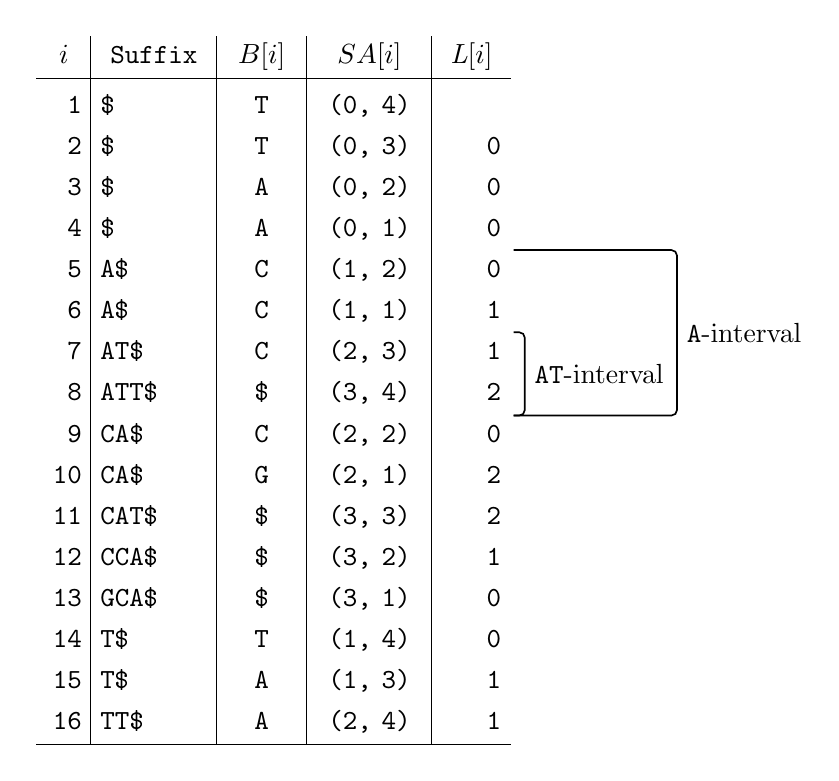
\begin{tikzpicture}
\matrix (m) [matrix of nodes,
nodes in empty cells,
text depth=0.4ex,text height=1.5ex,
nodes={font={\ttfamily},minimum height=1.3em},
column sep=0,row sep=0,
column 1/.style={nodes={text width=3ex, align=right}},
column 2/.style={nodes={text width=9ex, align=left}},
column 3/.style={nodes={text width=6ex, align=center}},
column 4/.style={nodes={text width=9ex, align=center}},
column 5/.style={nodes={text width=5ex, align=right}},
row 1/.style={nodes={align=center}}
]{
$i$ & Suffix & $B[i]$ & $SA[i]$ & $\LCP[i]$ \\[3pt]
1  & \$\color{grig}          &    T     & (0, 4) & \\
2  & \$\color{grig}          &    T     & (0, 3) & 0 \\
3  & \$\color{grig}          &    A     & (0, 2) & 0 \\
4  & \$\color{grig}          &    A     & (0, 1) & 0 \\
5  & A\$\color{grig}          &    C     & (1, 2) & 0 \\
6  & A\$\color{grig}          &    C     & (1, 1) & 1 \\
7  & AT\$\color{grig}          &    C     & (2, 3) & 1 \\
8  & ATT\$                     &    \$    & (3, 4) & 2 \\
9  & CA\$\color{grig}          &    C     & (2, 2) & 0 \\
10 & CA\$\color{grig}         &    G     & (2, 1) & 2 \\
11 & CAT\$                     &    \$    & (3, 3) & 2 \\
12 & CCA\$                     &    \$    & (3, 2) & 1 \\
13 & GCA\$                     &    \$    & (3, 1) & 0 \\
14 & T\$\color{grig}          &    T     & (1, 4) & 0 \\
15 & T\$\color{grig}          &    A     & (1, 3) & 1 \\
16 & TT\$\color{grig}          &    A     & (2, 4) & 1 \\
};

\draw (m-1-1.south west) -- (m-1-5.south east);
\draw (m-17-1.south west) -- (m-17-5.south east);
\foreach \y in {2,3,4,5} {
  \draw (m-1-\y.north west) -- (m-17-\y.south west);
};

\parentesi{m-6-5}{m-9-5}{6em}{$\mathtt{A}$-interval}{parentesi,rounded corners=2pt}{mid1}
\parentesi{m-8-5}{m-9-5}{0.5em}{$\mathtt{AT}$-interval}{parentesi,rounded corners=2pt}{mid2}
\end{tikzpicture}

\end{figure}

\end{document}